\chapter{Expérimentation}
\paragraph{}
Dans ce dernier chapitre du rapport, nous présenterons brièvement, dans un premier temps, les fonctions utilisées pour le calcul du temps pris par l’exécution d’un algorithme sur une donnée particulière, et pour le calcul d’espace mémoire total consommé par une structure de données. 
    
Et en deuxième lieu on effectuera des études expérimental de complexité en temps et on gain mémoire sur l'algorithme de compression et celui de la recherche.   

\section{Fonction pour le calcul du temps}
    Pour le calcul du temps pris par l'exécution d'un algorithme sur une donnée particulière, on utilise la fonction "\textit{gettimeofday ()}" du module \textbf{Unix} \cite{refUnix} de \textbf{OCaml}; une fonction qui nous renvoie l'heure actuelle avec une résolution supérieure à 1 seconde. Il suffit d'appeler la fonction avant et après l'algorithme, la temps donc c'est juste la différence entre les deux.
    
    Pour les résultats, on les met dans un fichier texte dans le but de les utiliser après avec l'application \textit{Gnuplot}\footnote{Gnuplot est un logiciel qui sert à produire des représentations graphiques en deux ou trois dimensions de fonctions numériques ou de données}
    
    L'implémentation de la fonction en \textbf{OCaml} est la suivante:
    \begin{minted}{ocaml} 
    let calculeTime donnees ... = 
      let out_channel = open_out "file" in
      .... 
        let start = Unix.gettimeofday () in 
        (* Exécution de l'algorithme *)
        fprintf out_channel "%fs \n" (Unix.gettimeofday () -. start); 
      ...
      close_out out_channel
    ;;
    \end{minted}
    
    
\section{Fonction pour le calcul d'espace mémoire}
    Il existe plusieurs façons pour le calcul d’espace mémoire total consommé par une structure de données, parmi elles on trouve le module \textbf{Gc}\cite{refGc} de \textbf{OCaml}. Gc présente plusieurs fonctions, mais dans ce rapport on se limitera à la fonction \textit{"Gc.stat()"} qui nous retourne un enregistrement possédant notamment les champs: 
    \begin{itemize}
        \item \textit{"minor\textunderscore words"}: le nombre de mots stocké dans le tas mineur
        \item \textit{"major\textunderscore words"}: le nombre de mots stocké dans le tas majeur
        \item \textit{"promoted\textunderscore words"}: le nombre de mots qui on été promu du tas mineur au tas majeur
    \end{itemize}
    Le calcul de l'occupation mémoire s'effectue de la façon suivante :  \textit{heap\textunderscore allocation = minor\textunderscore words + major\textunderscore words - promoted\textunderscore words}
    Les résultats seront comme pour la fonction précédente fournis dans un fichier attaché à l'archive.
    \\ \\ \\
    \\L'implémentation est la suivante:
    \begin{minted}{ocaml} 
    let calculeMemory donnees ... = 
      let out_channel = open_out "file" in
      .... 
        let start = ( (Gc.stat()).minor_words +. (Gc.stat()).major_words 
        -. (Gc.stat()).promoted_words ) in
            (* Construction/affectation de la structure de données *)
        let end = ( (Gc.stat()).minor_words +. (Gc.stat()).major_words 
        -. (Gc.stat()).promoted_words ) in
        let m =  int_of_float(end -. start) in 
        fprintf out_channel "%fs \n" (m); 
      ...
      close_out out_channel
    ;;
    \end{minted} 


\section{Étude expérimentale de complexité en temps des algorithmes de recherche}
Dans cette étude, on effectuera (2 x (La taille de l'ABR)) recherche et on prendra à la fin la moyen des temps de recherche de la totalité des recherches; avec cette approche on garantit \textit{presque} la correction du résultat  
Pour les tailles des arbres à générer, ça sera des arbre de 1000 à nb * 1000 avec "nb" une donnée pour l'algorithme d'expérimentation.  
Par exemple avec nb=18 on aura le résultat suivant:
\begin{center}
    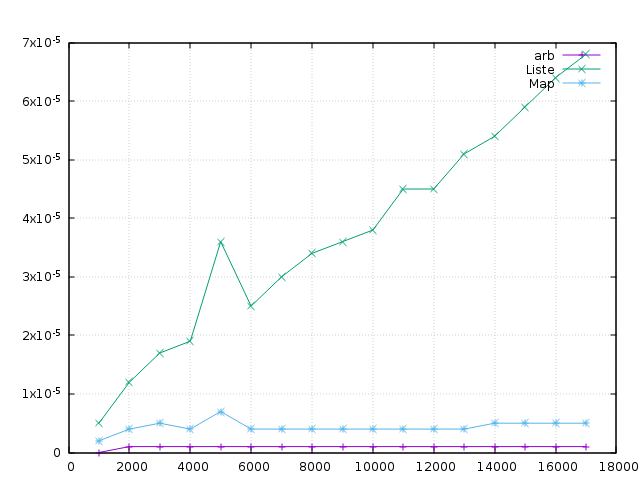
\includegraphics[scale=0.8]{assets/rechercheTests.png}
    \caption{\\ Le temps des algorithmes de recherche}
\end{center}
On remarque, avec ce graphe que la complexité de recherche théorique correspond à peu près aux résultats que l'on obtient. En effet avec l'implémentation en liste, On perd beaucoup en efficacité de recherche contrairement à l'implémentation à l'aide d'une Map ou la recherche n'est pas très impactée.

\section{Étude expérimentale de complexité en espace}
Dans cette partie, on s'intéresse à la consommation mémoire de nos structures de données. Notre étude se fera sur des arbres de recherches de taille 1000 à 180000, et nous étudierons l'occupation dans le tas comme décrit dans la partie précédente.
\begin{center}
    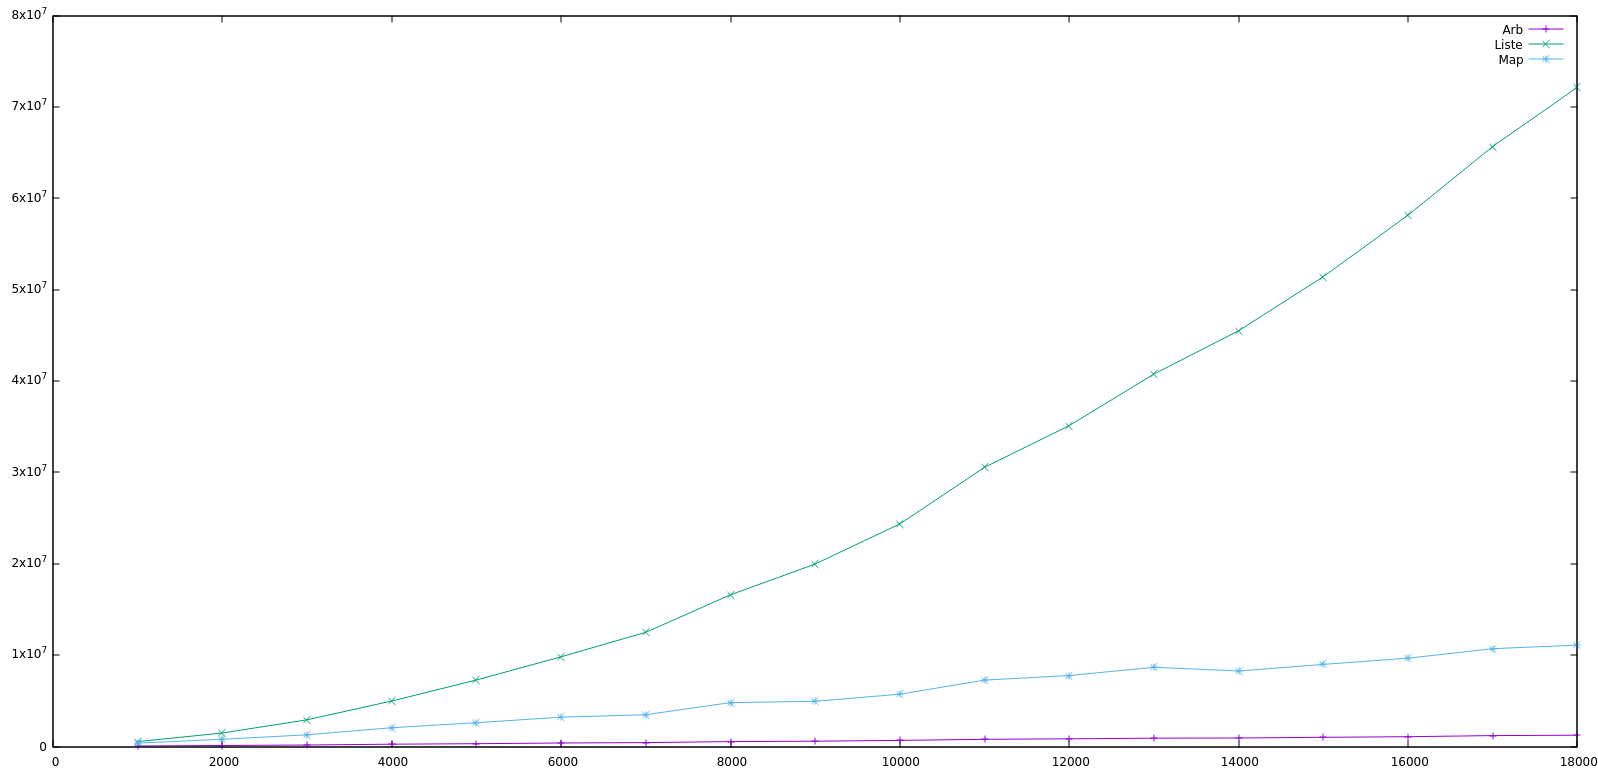
\includegraphics[scale=0.38]{assets/memory_alm.png}
    \caption{\\ Mémoire utilisée par structure}
\end{center}

Contrairement à nos attentes, la consommation mémoire est du loin supérieure pour un arbre compressé (que ce soit avec des listes ou des maps) que pour un arbre binaire standard.

\paragraph{}
Dans ce qui suit, on s'intéressera plus aux arbres compressés avec des maps et aux ABR.

\begin{center}
    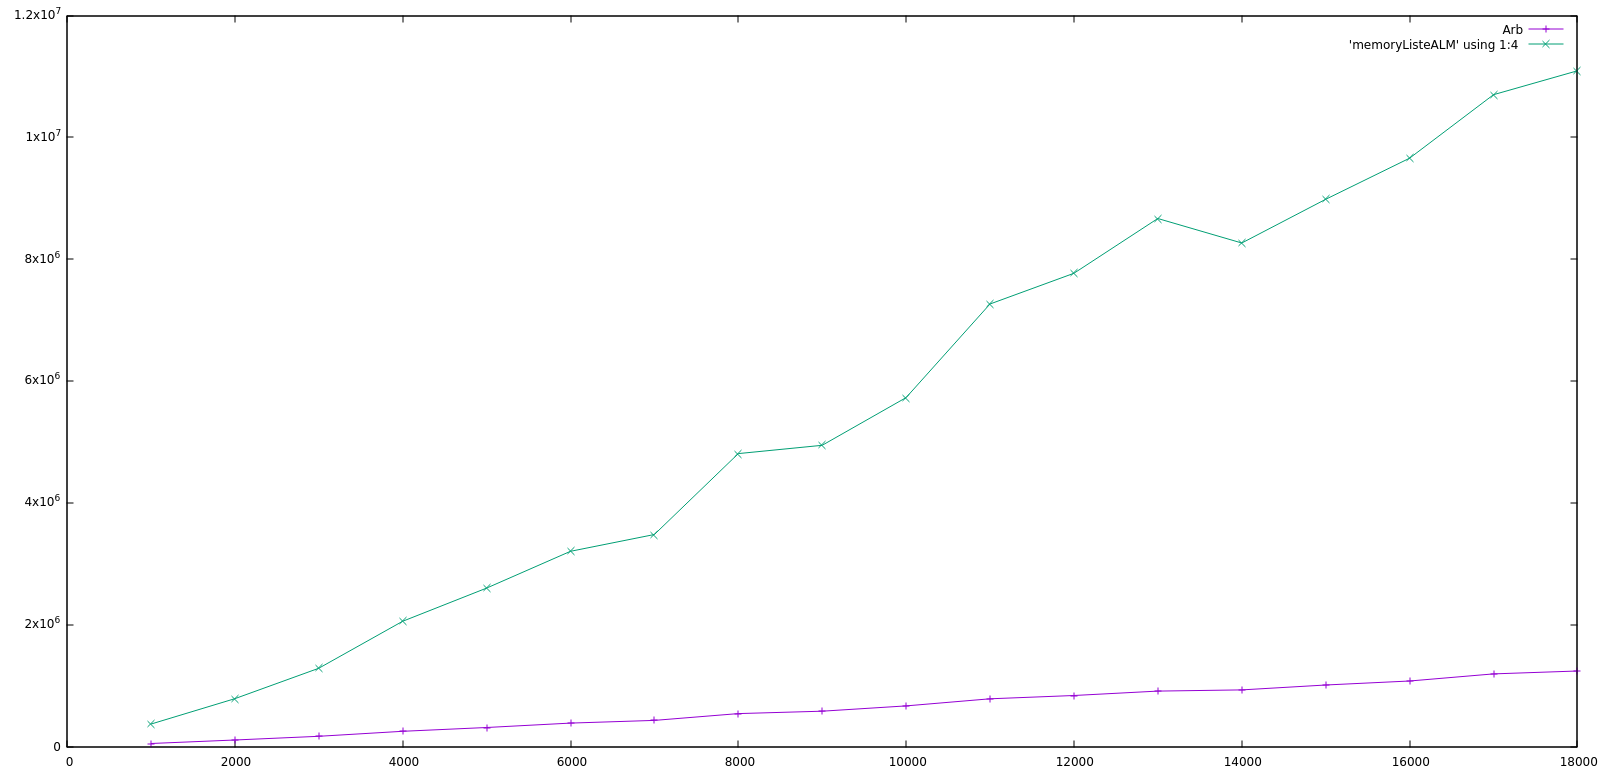
\includegraphics[scale=0.38]{assets/memory_am.png}
    \caption{\\ Mémoire utilisée par la map et l'ABR}
\end{center}
Comme on peut le voir plus précisément dans ce graphe, il y a une grande différence entre notre implémentation des arbres compressés avec des Map et et celle des ABR.


    
\section{Étude expérimentale sur le taux de compression }
\subsection{Nombre de nœuds internes}
Cette fois-ci, on étudiera de près le nombre de nœuds internes dans les arbres compressés avec des listes obtenus avec le jeu de test donné\footnote{\url{https://www-apr.lip6.fr/~genitrini/doc\_ens/Jeu\_de\_tests.tar.gz}}.

\begin{center}
\begin{tabular}{| g | d |}
    \hline
     Nombres de valeurs & Nombres de noeuds internes \\
    \hline
     100 & 100 \\
     150 & 59 \\
     500 & 176 \\
     750 & 258 \\
     1000 & 1000 \\
    10000 & 2497 \\
    50000 & 10846 \\
    \hline
    \end{tabular}    
\end{center}
En plus de cela, nous avons effectuer des tests sur des données aléatoires, présentés dans le graphe ci-dessous.
\begin{center}
    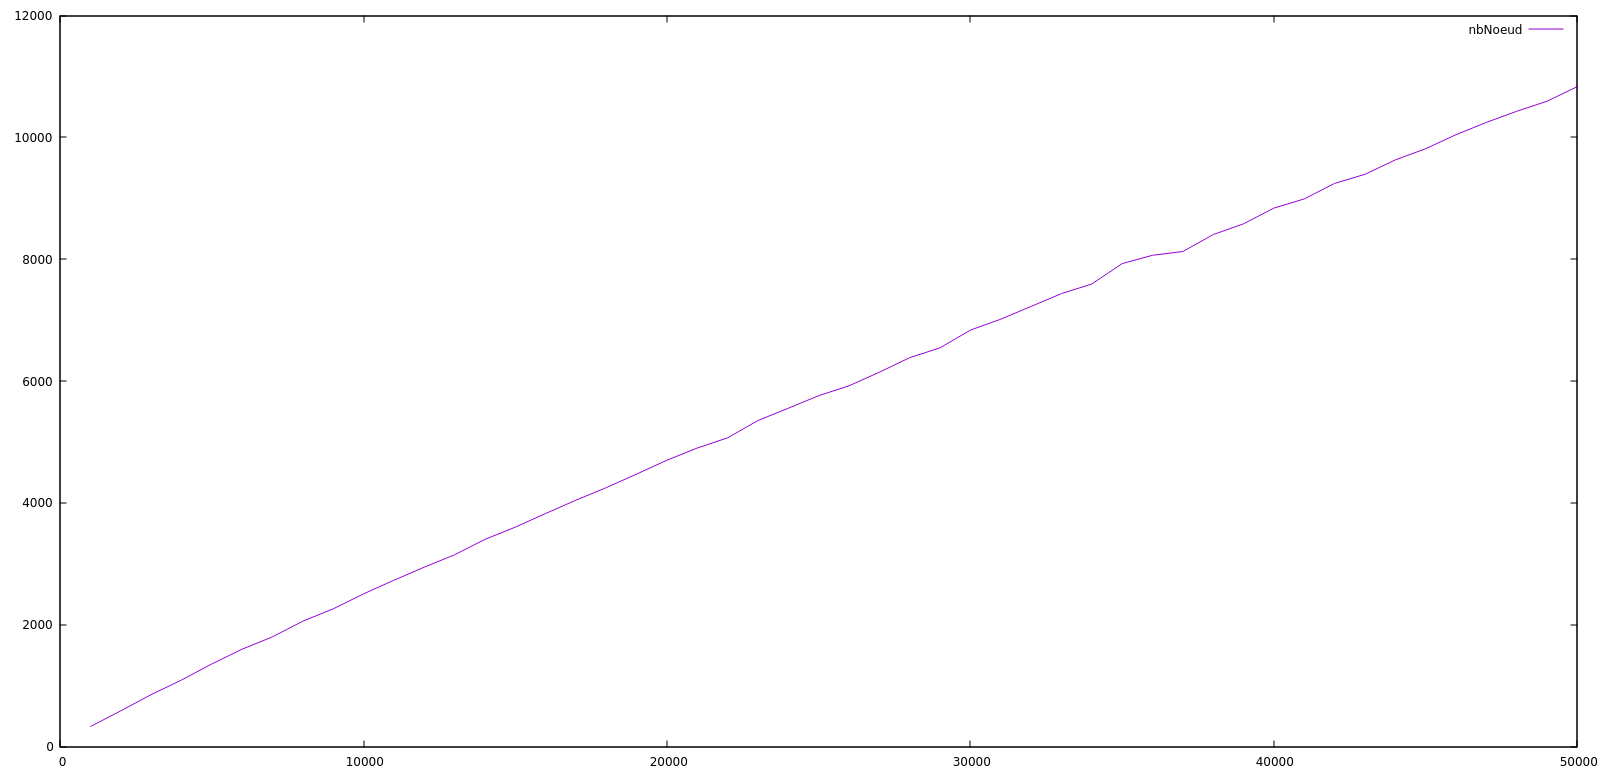
\includegraphics[scale=0.38]{assets/graphe_nb_noeuds.png}
    \caption{\\ Nombre de nœuds internes}
\end{center}

\subsection{Nombre moyen de clés par nœud interne}
On étudiera maintenant le nombre moyen de clés par nœud interne dans les arbres compressés avec des lites, obtenus avec le jeu de test donné.
\\
\begin{center}
\begin{tabular}{| g | d |}
    \hline
     Nombres de valeurs & Nombres de valeurs par noeud \\
    \hline
    100 & 1.0 \\
    150 & 2.5 \\
    500 & 2.8 \\
    750 & 2.9 \\
    1000 & 1.0 \\
    10000 & 4.0 \\
    50000 & 4.6 \\
    \hline
    \end{tabular}    
\end{center}

\paragraph{} \vspace{1,9cm}
Comme précédemment, on a aussi fait d'autres tests sur des arbres aléatoires:
\begin{center}
    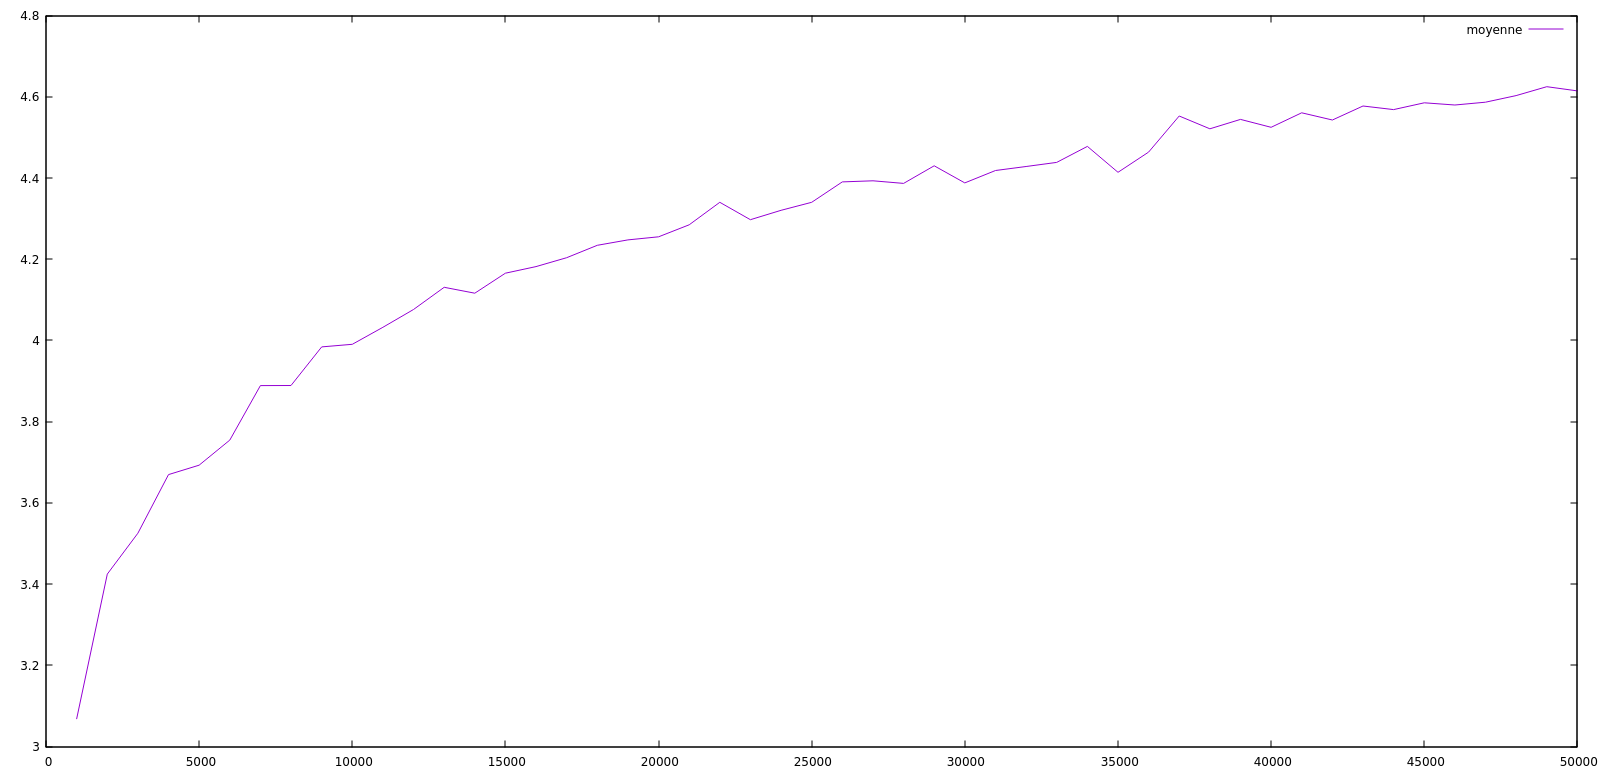
\includegraphics[scale=0.38]{assets/graphe_moyenne_noeuds.png}
    \caption{\\ Nombre moyen de clés par nœud interne}
\end{center}